% https://www.r-bloggers.com/2012/02/r-and-presentations-a-basic-example-of-knitr-and-beamer/

\documentclass{beamer}\usepackage[]{graphicx}\usepackage[]{xcolor}
% maxwidth is the original width if it is less than linewidth
% otherwise use linewidth (to make sure the graphics do not exceed the margin)
\makeatletter
\def\maxwidth{ %
  \ifdim\Gin@nat@width>\linewidth
    \linewidth
  \else
    \Gin@nat@width
  \fi
}
\makeatother

\definecolor{fgcolor}{rgb}{0.345, 0.345, 0.345}
\newcommand{\hlnum}[1]{\textcolor[rgb]{0.686,0.059,0.569}{#1}}%
\newcommand{\hlsng}[1]{\textcolor[rgb]{0.192,0.494,0.8}{#1}}%
\newcommand{\hlcom}[1]{\textcolor[rgb]{0.678,0.584,0.686}{\textit{#1}}}%
\newcommand{\hlopt}[1]{\textcolor[rgb]{0,0,0}{#1}}%
\newcommand{\hldef}[1]{\textcolor[rgb]{0.345,0.345,0.345}{#1}}%
\newcommand{\hlkwa}[1]{\textcolor[rgb]{0.161,0.373,0.58}{\textbf{#1}}}%
\newcommand{\hlkwb}[1]{\textcolor[rgb]{0.69,0.353,0.396}{#1}}%
\newcommand{\hlkwc}[1]{\textcolor[rgb]{0.333,0.667,0.333}{#1}}%
\newcommand{\hlkwd}[1]{\textcolor[rgb]{0.737,0.353,0.396}{\textbf{#1}}}%
\let\hlipl\hlkwb

\usepackage{framed}
\makeatletter
\newenvironment{kframe}{%
 \def\at@end@of@kframe{}%
 \ifinner\ifhmode%
  \def\at@end@of@kframe{\end{minipage}}%
  \begin{minipage}{\columnwidth}%
 \fi\fi%
 \def\FrameCommand##1{\hskip\@totalleftmargin \hskip-\fboxsep
 \colorbox{shadecolor}{##1}\hskip-\fboxsep
     % There is no \\@totalrightmargin, so:
     \hskip-\linewidth \hskip-\@totalleftmargin \hskip\columnwidth}%
 \MakeFramed {\advance\hsize-\width
   \@totalleftmargin\z@ \linewidth\hsize
   \@setminipage}}%
 {\par\unskip\endMakeFramed%
 \at@end@of@kframe}
\makeatother

\definecolor{shadecolor}{rgb}{.97, .97, .97}
\definecolor{messagecolor}{rgb}{0, 0, 0}
\definecolor{warningcolor}{rgb}{1, 0, 1}
\definecolor{errorcolor}{rgb}{1, 0, 0}
\newenvironment{knitrout}{}{} % an empty environment to be redefined in TeX

\usepackage{alltt}

% pacotes
% \usepackage{Sweave} % para usar o Sweave, oras
% \SweaveOpts{concordance=FALSE} % para chamar outros arquivos Rnw, conforme https://support.rstudio.com/hc/en-us/articles/200486298-Working-with
\usepackage[brazil]{babel} % sudo tlmgr install babel-brazil   % sudo tlmgr update --self  % sudo tlmgr install babel-portuges
\usepackage[utf8]{inputenc}
\usepackage{fancybox}
\usepackage{textpos}  % sudo tlmgr install textpos
\usepackage{hyperref} % \href
\usepackage{tcolorbox} % para caixas coloridas  % sudo tlmgr install tcolorbox


% Blind footnotes
\newcommand\blfootnote[1]{%
  \begingroup
  \renewcommand\thefootnote{}\footnote{#1}%
  \addtocounter{footnote}{-1}%
  \endgroup
}

% bibliografia
% \bibliographystyle{plain}
% \bibliography{mp.bib}

% configuração dos links
\hypersetup
{
colorlinks=true,
linkcolor=blue,
urlcolor=blue,
filecolor=blue,
linktoc=all,
}

% pasta de imagens
\graphicspath{{./img/}}


% conteúdo
\title{Modelagem Preditiva}
\author{Filipe J. Zabala}
\institute{\href{https://www.pucrs.br/politecnica/}{Escola Politécnica} \\
           \href{https://www.pucrs.br/}{PUCRS} \\
           \texttt{\href{http://filipezabala.com}{filipezabala.com}}}
\date{2024-08-09}

\usetheme{Pittsburgh}
% \usecolortheme{owl} % sudo tlmgr install beamercolorthemeowl

% logo
\addtobeamertemplate{frametitle}{}{%
\begin{textblock*}{10mm}(-.05\textwidth,-.85cm)

\includegraphics[width=2cm]{logo_politecnica.png}
\end{textblock*}}
\IfFileExists{upquote.sty}{\usepackage{upquote}}{}
\begin{document}
\frame{\titlepage}

\begin{frame}
    \frametitle{Sumário}
    \tableofcontents
\end{frame}

\section{Minibio}
\begin{frame}{\secname}
Filipe J. Zabala $\cdot$ \url{filipe.zabala@pucrs.br}
\vspace{1cm}
  \begin{itemize}
    \item 2000-2004 Bacharel em Estatística \href{https://lume.ufrgs.br/handle/10183/130892}{IME-UFRGS}
    \item 2006-2009 Mestre em Estatística \href{https://www.teses.usp.br/teses/disponiveis/45/45133/tde-01032021-140004/pt-br.php}{IME-USP}
    \item 2007-2009 Analista do \href{https://www.itau.com.br/}{Banco Itaú S.A.}
    \item 2009-$\hphantom{2021}$ Sócio da \href{https://filipezabala.com/}{ZN Consultoria Estatística}
    \item 2010-$\hphantom{2021}$ Professor da \href{https://portal.pucrs.br/ensino/escola-politecnica/}{Escola Politécnica da PUCRS}
    \item 2019-$\hphantom{2024}$ Doutorando no \href{https://www.ufrgs.br/ppgpsiquiatria/}{PPG Psiquiatria e C.C. UFRGS}
  \end{itemize}
\end{frame}


\section{Para começar}
\begin{frame}{\secname}
    \begin{itemize}
    \item \textit{Every once in a while there is house cleaning in mathematics. Some old names are discarded, some dusted off and refurbished; new theories, new additions to the household are assigned a place and name.} Kasner and Newman (1940,3)
    \pause
    \item Estatística \textit{vs} Ciência de Dados \textit{vs} Analytics \textit{vs} IA \textit{vs} ...
    \pause
    \item Teoria da Decisão \textit{vs} Aprendizado por Reforço \textit{vs} Aprendizado de Máquina
    \pause
    \item Maximizar a utilidade esperada \textit{vs} Maximizar a recompensa \textit{vs} Minimizar o erro
    \end{itemize}
\end{frame}

\section{Sobre modelagem preditiva}
\begin{frame}{\secname}
    \begin{itemize}
    \item Do Latim \textit{praedicere}, anunciar antecipadamente
    \pause
    \item Métodos para predizer novos valores de $X$
      \begin{itemize}
      \item $X$: variável de interesse
      \item $\theta$: parâmetro associado a $X$
      \end{itemize}
    \pause
    \item \textit{As duas culturas} de Leo Breiman (2001):
      \begin{itemize}
      \item interpretar $\theta$ \textit{vs} predizer $X$
      \end{itemize}
    % \pause
    % \item Bruno de Finetti (1974): \textit{Probability, like beauty, exists only in the mind.}
    \pause
    \item Debabrata Basu (1988): \textit{Information is what information does. It changes opinion (about $\theta$).}
    \pause
    \item George Box (1979): \textit{All models are wrong but some are useful.}
    \end{itemize}
\end{frame}


\section{Inferência bayesiana}
\begin{frame}{\secname}
    \begin{itemize}
    \item Priori: opinião (sobre $\theta$) em forma de probabilidade antes de observar os dados \[ \pi(\theta) \]
    \pause
    \item Verossimilhança: função (de $\theta$) com informação dos dados \[ L(\theta|x) \]
    \pause
    \item Posteriori: opinião (sobre $\theta$) em forma de probabilidade depois de observar os dados \[ \pi(\theta|x) \]
    \end{itemize}
\end{frame}


\begin{frame}{\secname}
    \begin{itemize}
    \item Operação bayesiana: calibrar a opinião à luz dos dados \[ \pi(\theta|x) = \frac{\pi(\theta) L(\theta|x)}{P(X=x)} \]
    % \pause
    % \item Independência condicional (em relação a $\theta$)
    \pause
    \item `A posteriori de hoje é a priori de amanhã' (Máxima bayesiana)
    \pause
    \item Preditiva: distribuição de $X$ \[ P(X=x) = \int_{\theta} \pi(\theta) L(\theta|x) d\theta \]
    \pause
    \item A probabilidade de o próximo resultado da moeda ser `cara` \[ Pr(X_{n+1}=\textrm{cara}) = \frac{r+1}{n+2} \]
    \end{itemize}
\end{frame}

% \section{Inferência bayesiana}
\begin{frame}{\secname}
    \begin{itemize}
    \item Variáveis permutáveis: a ordem das observações é indiferente \[ Pr(X_1=x_1, \ldots, X_N=x_N) = Pr(X_{\pi(1)}=x_1, \ldots, X_{\pi(N)}=x_N)  \]
    \pause
    \item Teorema da representação de de Finetti (1930) \[ Pr(X_1=x_1, \ldots, X_N=x_N) = \int_{\theta} \theta^a (1-\theta)^b \mu(d\theta) \]
    \pause
    \item Flexibiliza a suposição de independência
    \pause
    \item Trata $\theta$ apenas como uma variável de integração
    \end{itemize}
\end{frame}


\section{Exemplos}
\begin{frame}{Ex. 1: Previsão de demanda}
  \begin{itemize}
  \item Objetivo: prever a demanda de bebida em função da temperatura máxima do dia
  \item \href{https://filipezabala.com/eb/rls.html}{Seção 7.2} de \href{https://filipezabala.com/eb}{Zabala (2024) - Estatística Básica}
  \item $Y$: número de garrafas de bebida consumidas
  \item $X$: temperatura máxima do dia em $^{\circ}{\rm C}$
  \item Modelo: $y = \hat{\beta}_0 + \hat{\beta}_1 x$
  \end{itemize}
\end{frame}

\begin{frame}[fragile]{Ex. 1: Previsão de demanda}
\fontsize{8pt}{8pt}\selectfont
Obtendo dados e estatísticas descritivas.
\begin{knitrout}
\definecolor{shadecolor}{rgb}{0.969, 0.969, 0.969}\color{fgcolor}\begin{kframe}
\begin{alltt}
\hldef{dr} \hlkwb{<-} \hlkwd{read.table}\hldef{(}\hlsng{'https://filipezabala.com/data/drinks.txt'}\hldef{,}
                 \hlkwc{header} \hldef{=} \hlnum{TRUE}\hldef{)}
\hlkwd{str}\hldef{(dr)}  \hlcom{# estrutura dos dados}
\end{alltt}
\begin{verbatim}
## 'data.frame':	30 obs. of  2 variables:
##  $ temp: num  29.5 31.3 34.7 40.4 28.4 40.3 41.1 36.2 35.7 26.1 ...
##  $ gar : int  146 170 167 244 159 195 225 206 200 134 ...
\end{verbatim}
\begin{alltt}
\hlkwd{summary}\hldef{(dr)}
\end{alltt}
\begin{verbatim}
##       temp            gar       
##  Min.   :25.20   Min.   :106.0  
##  1st Qu.:29.50   1st Qu.:161.0  
##  Median :32.55   Median :178.5  
##  Mean   :33.66   Mean   :180.0  
##  3rd Qu.:37.88   3rd Qu.:199.8  
##  Max.   :41.90   Max.   :244.0
\end{verbatim}
\end{kframe}
\end{knitrout}
\end{frame}

\begin{frame}[fragile]{Ex. 1: Previsão de demanda}
\fontsize{8pt}{8pt}\selectfont
\begin{knitrout}
\definecolor{shadecolor}{rgb}{0.969, 0.969, 0.969}\color{fgcolor}\begin{kframe}
\begin{alltt}
\hlkwd{plot}\hldef{(dr,} \hlkwc{xlab} \hldef{=} \hlsng{'Temperatura máxima'}\hldef{,} \hlkwc{ylab} \hldef{=} \hlsng{'Número de garrafas'}\hldef{,}
     \hlkwc{cex} \hldef{=} \hlnum{1.3}\hldef{,} \hlkwc{cex.axis} \hldef{=} \hlnum{1.3}\hldef{,} \hlkwc{cex.lab} \hldef{=} \hlnum{1.3}\hldef{)}
\hlkwd{legend}\hldef{(}\hlnum{26}\hldef{,} \hlnum{235}\hldef{,} \hlkwc{legend}\hldef{=}\hlkwd{paste0}\hldef{(}\hlsng{'r = '}\hldef{,} \hlkwd{round}\hldef{(}\hlkwd{cor}\hldef{(dr}\hlopt{$}\hldef{temp,dr}\hlopt{$}\hldef{gar),}\hlnum{3}\hldef{)),}
       \hlkwc{cex} \hldef{=} \hlnum{1.2}\hldef{,} \hlkwc{box.lty} \hldef{=} \hlnum{0}\hldef{)}
\end{alltt}
\end{kframe}

{\centering 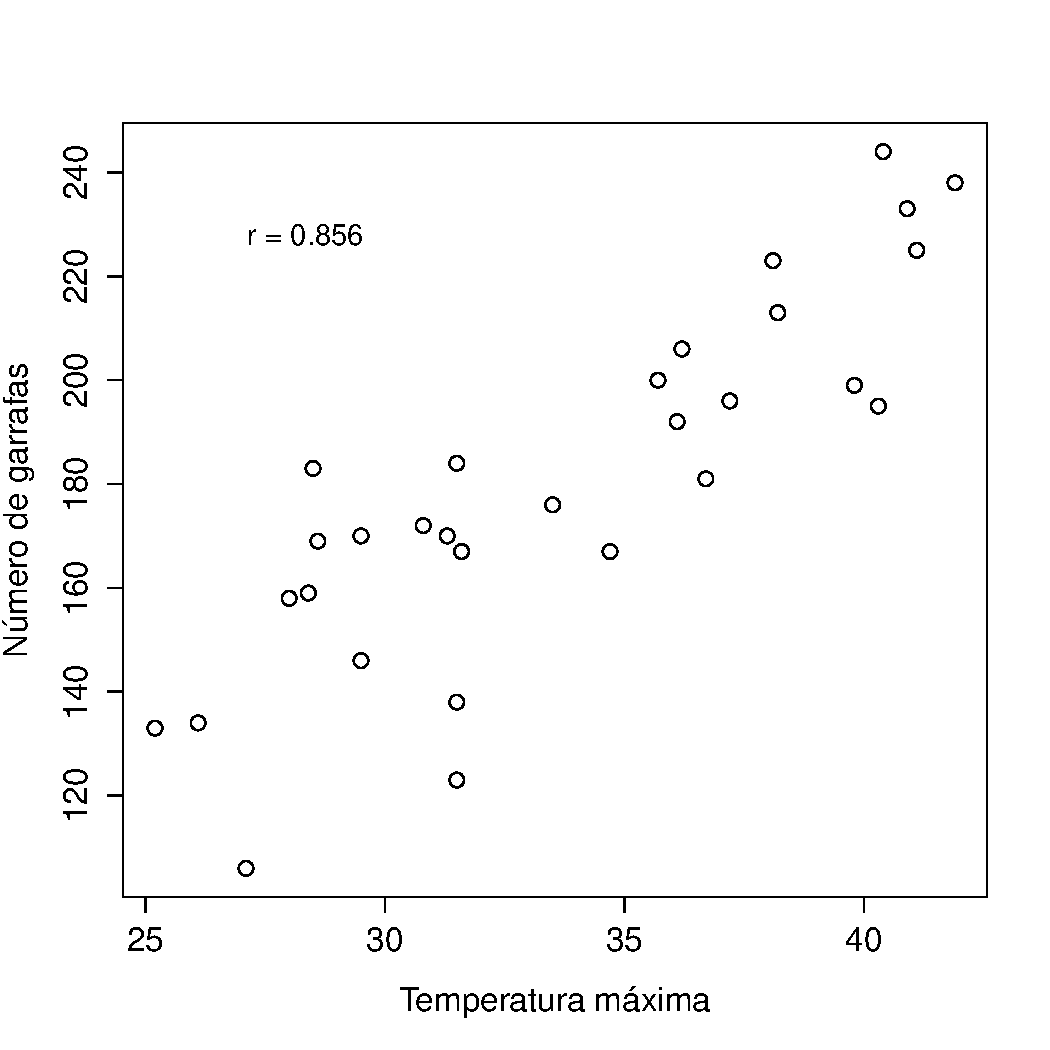
\includegraphics[width=.6\linewidth]{figure/plot_base-1} 

}


\end{knitrout}
\end{frame}

\begin{frame}[fragile]{Ex. 1: Previsão de demanda}
\fontsize{8pt}{8pt}\selectfont
\begin{knitrout}
\definecolor{shadecolor}{rgb}{0.969, 0.969, 0.969}\color{fgcolor}\begin{kframe}
\begin{alltt}
\hldef{fit} \hlkwb{<-} \hlkwd{lm}\hldef{(gar} \hlopt{~} \hldef{temp,} \hlkwc{data} \hldef{= dr)} \hlcom{# modelo clássico}
\hlkwd{summary}\hldef{(fit)}
\end{alltt}
\begin{verbatim}
## 
## Call:
## lm(formula = gar ~ temp, data = dr)
## 
## Residuals:
##     Min      1Q  Median      3Q     Max 
## -44.204  -8.261   3.518  10.796  33.540 
## 
## Coefficients:
##             Estimate Std. Error t value Pr(>|t|)    
## (Intercept) -19.1096    22.9195  -0.834    0.411    
## temp          5.9147     0.6736   8.780 1.57e-09 ***
## ---
## Signif. codes:  0 '***' 0.001 '**' 0.01 '*' 0.05 '.' 0.1 ' ' 1
## 
## Residual standard error: 18.24 on 28 degrees of freedom
## Multiple R-squared:  0.7336,	Adjusted R-squared:  0.7241 
## F-statistic:  77.1 on 1 and 28 DF,  p-value: 1.565e-09
\end{verbatim}
\begin{alltt}
\hldef{(pr} \hlkwb{<-} \hlkwd{predict}\hldef{(fit,} \hlkwc{newdata} \hldef{=} \hlkwd{data.frame}\hldef{(}\hlkwc{temp} \hldef{=} \hlnum{39}\hldef{)))}
\end{alltt}
\begin{verbatim}
##        1 
## 211.5649
\end{verbatim}
\end{kframe}
\end{knitrout}
\end{frame}

\begin{frame}[fragile]{Ex. 1: Previsão de demanda}
\fontsize{8pt}{8pt}\selectfont
\begin{knitrout}
\definecolor{shadecolor}{rgb}{0.969, 0.969, 0.969}\color{fgcolor}\begin{kframe}
\begin{alltt}
\hlkwd{plot}\hldef{(dr,} \hlkwc{xlab} \hldef{=} \hlsng{'Temperatura máxima'}\hldef{,} \hlkwc{ylab} \hldef{=} \hlsng{'Número de garrafas'}\hldef{,}
     \hlkwc{cex} \hldef{=} \hlnum{1.3}\hldef{,} \hlkwc{cex.axis} \hldef{=} \hlnum{1.3}\hldef{,} \hlkwc{cex.lab} \hldef{=} \hlnum{1.3}\hldef{)}
\hlkwd{abline}\hldef{(fit}\hlopt{$}\hldef{coefficients[}\hlnum{1}\hldef{], fit}\hlopt{$}\hldef{coefficients[}\hlnum{2}\hldef{],} \hlkwc{col} \hldef{=} \hlsng{'red'}\hldef{)}
\hlkwd{abline}\hldef{(}\hlkwc{v} \hldef{=} \hlnum{39}\hldef{,} \hlkwc{col} \hldef{=} \hlsng{'blue'}\hldef{,} \hlkwc{lty} \hldef{=} \hlnum{2}\hldef{)}
\hlkwd{abline}\hldef{(}\hlkwc{h} \hldef{= pr,} \hlkwc{col} \hldef{=} \hlsng{'blue'}\hldef{,} \hlkwc{lty} \hldef{=} \hlnum{2}\hldef{)}
\end{alltt}
\end{kframe}

{\centering 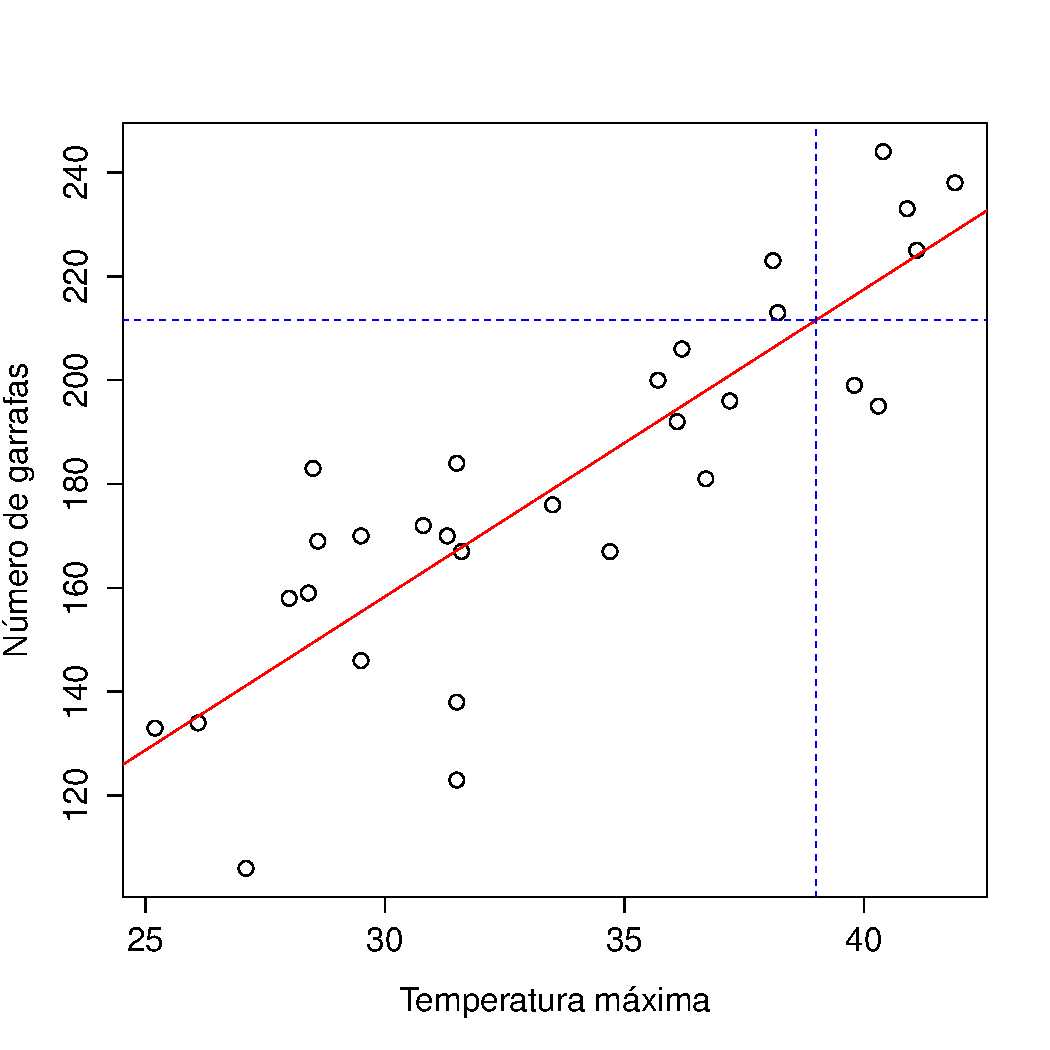
\includegraphics[width=.6\linewidth]{figure/abline-1} 

}


\end{knitrout}
\end{frame}

\begin{frame}[fragile]{Ex. 1: Previsão de demanda}
\fontsize{8pt}{8pt}\selectfont
\begin{knitrout}
\definecolor{shadecolor}{rgb}{0.969, 0.969, 0.969}\color{fgcolor}\begin{kframe}
\begin{alltt}
\hlcom{# modelo bayesiano}
\hlkwd{options}\hldef{(}\hlkwc{mc.cores} \hldef{= parallel}\hlopt{::}\hlkwd{detectCores}\hldef{())}
\hldef{fit_stan} \hlkwb{<-} \hldef{rstanarm}\hlopt{::}\hlkwd{stan_glm}\hldef{(gar} \hlopt{~} \hldef{temp,} \hlkwc{data} \hldef{= dr,} \hlkwc{family} \hldef{= gaussian)}
\hldef{fit_stan}
\end{alltt}
\begin{verbatim}
## stan_glm
##  family:       gaussian [identity]
##  formula:      gar ~ temp
##  observations: 30
##  predictors:   2
## ------
##             Median MAD_SD
## (Intercept) -18.9   23.1 
## temp          5.9    0.7 
## 
## Auxiliary parameter(s):
##       Median MAD_SD
## sigma 18.6    2.4  
## 
## ------
## * For help interpreting the printed output see ?print.stanreg
## * For info on the priors used see ?prior_summary.stanreg
\end{verbatim}
\end{kframe}
\end{knitrout}
\end{frame}


\begin{frame}[fragile]{Ex. 1: Previsão de demanda}
\textit{If the model fits, then replicated data generated under the model should look similar to observed data.} Gelman et al (2013,143)
\fontsize{8pt}{8pt}\selectfont
\begin{knitrout}
\definecolor{shadecolor}{rgb}{0.969, 0.969, 0.969}\color{fgcolor}\begin{kframe}
\begin{alltt}
\hldef{rstanarm}\hlopt{::}\hlkwd{pp_check}\hldef{(fit_stan)} \hlcom{# posterior predictive checking}
\end{alltt}
\end{kframe}

{\centering 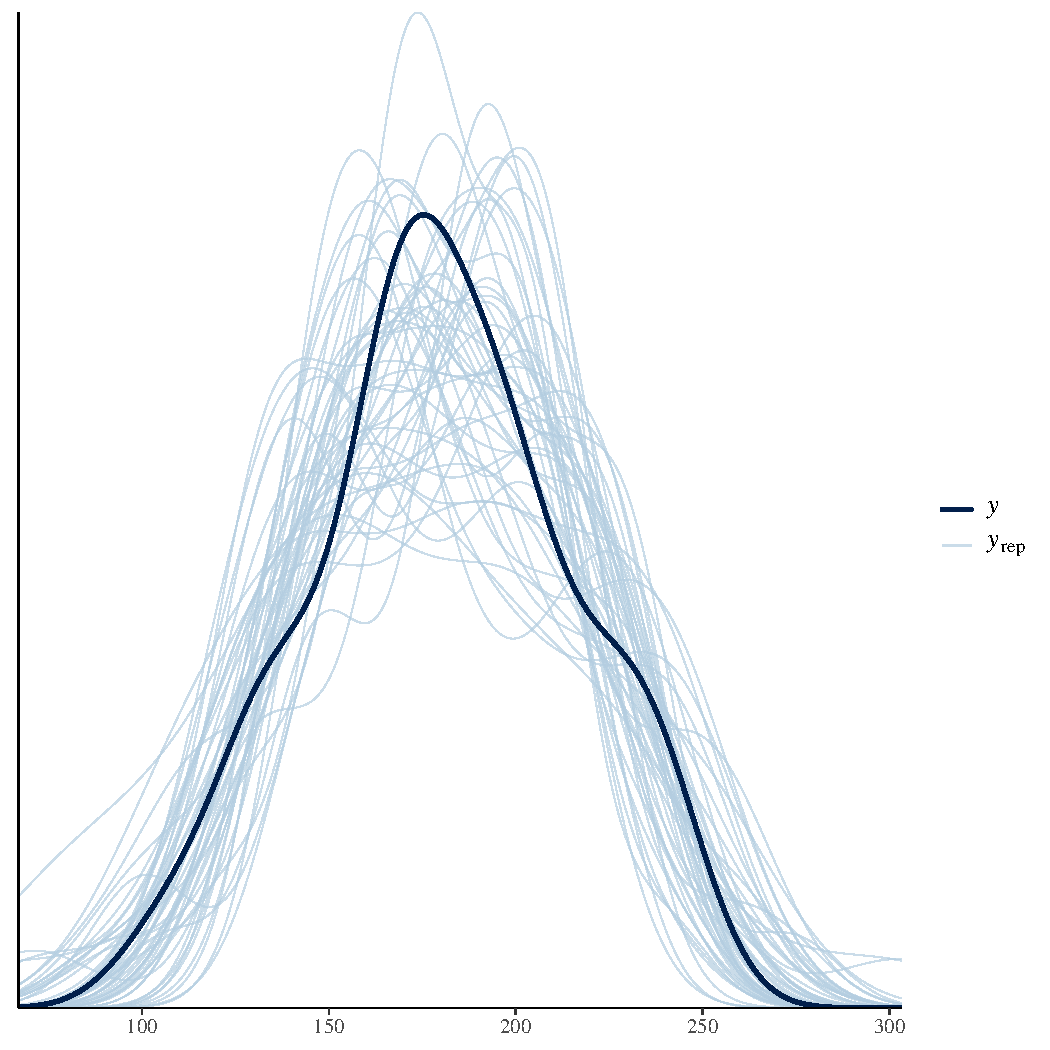
\includegraphics[width=.5\linewidth]{figure/ppc-1} 

}


\end{knitrout}
\end{frame}



\begin{frame}[fragile]{Ex. 2: Previsão de volume processual}
  \begin{itemize}
  \item \href{https://github.com/filipezabala/jurimetrics/}{\texttt{jurimetrics}}: ferramentas para \href{https://ww2.esmarn.tjrn.jus.br/revistas/index.php/revista\_direito\_e\_liberdade/article/view/732}{Jurimetria} %\cite{zabala2024jurimetrics}
  \pause
  \item \texttt{tjrs\_2000\_2017}: série mensal de jan/2000 a dez/2017 da cota inferior de volume processual no segundo grau do TJ-RS
  \end{itemize}
\fontsize{6pt}{6pt}\selectfont  
\begin{knitrout}
\definecolor{shadecolor}{rgb}{0.969, 0.969, 0.969}\color{fgcolor}\begin{kframe}
\begin{alltt}
\hldef{jurimetrics}\hlopt{::}\hldef{tjrs_00_17}\hlopt{$}\hldef{count_adjusted}
\end{alltt}
\begin{verbatim}
##        Jan   Feb   Mar   Apr   May   Jun   Jul   Aug   Sep   Oct   Nov   Dec
## 2000    10   199   517   581   987  2074    96  4264  2967  3824  4510  4332
## 2001   197  2832  4334  3644  5275  4571   178  5638  3558  4330  4804  4824
## 2002   196  2863  4309  4326  5359  5447   266  5317  4546  7253  8607 11955
## 2003  1162  7845 11361 12819 12804 15229   856 16947 15460 18073 16656 18377
## 2004   677 10013 22227 18562 18420 22918  3314 21522 20948 19164 19747 23187
## 2005   683 10787 23602 20146 19612 26153 16213 23389 21239 19886 22740 23127
## 2006 14199 10986 24322 22791 25609 25769 20681 30839 24275 25657 29061 28746
## 2007  6447 19618 30692 26569 31335 27542 24096 33065 27126 30646 29016 26661
## 2008 11490 18158 29504 30598 29892 31958 30728 40828 34408 41238 35749 30162
## 2009 16367 15698 38680 38735 32054 37082 34679 38500 39260 36593 35815 29585
## 2010 20663 18758 39455 34965 40298 33780 35349 36246 34999 34714 35417 31460
## 2011 17990 24421 33980 32770 34319 38069 32344 40096 36581 34035 33303 30798
## 2012 15440 21913 38503 33899 41206 36746 28989 41048 31124 39001 33790 29317
## 2013 14693 19745 34876 35865 34252 35780 28517 37606 32825 38911 34410 28663
## 2014 14497 20139 30409 33173 33156 24049 31945 36489 34256 38395 33705 33406
## 2015 15362 26139 36961 35838 30456 33209 32480 34602 34688 19377 40370 27943
## 2016 12086 20802 31884 26466 29055 38739 33769 38571 34335 34177 34116 28583
## 2017  7754 24462 39869 28881 32684 30093 30144 36987 29486 33621 33241 26020
\end{verbatim}
\end{kframe}
\end{knitrout}
\end{frame}

\begin{frame}[fragile]{Ex. 2: Previsão de volume processual}
\fontsize{8pt}{8pt}\selectfont
\begin{knitrout}
\definecolor{shadecolor}{rgb}{0.969, 0.969, 0.969}\color{fgcolor}\begin{kframe}
\begin{alltt}
\hlkwd{library}\hldef{(jurimetrics)}
\hldef{y} \hlkwb{<-} \hlkwd{ts}\hldef{(tjrs_00_17}\hlopt{$}\hldef{count_adjusted,} \hlkwc{start} \hldef{=} \hlkwd{c}\hldef{(}\hlnum{2000}\hldef{,}\hlnum{1}\hldef{),} \hlkwc{frequency} \hldef{=} \hlnum{12}\hldef{)}
\hlkwd{fits}\hldef{(y,} \hlkwc{show.sec.graph} \hldef{=} \hlnum{FALSE}\hldef{,} \hlkwc{show.value} \hldef{=} \hlnum{FALSE}\hldef{)}
\end{alltt}
\end{kframe}
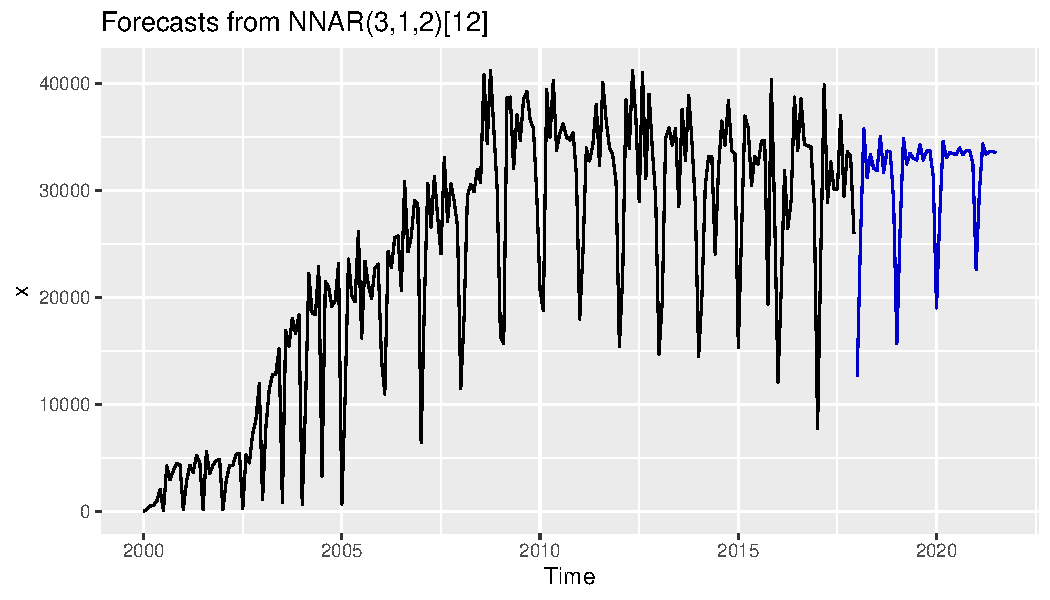
\includegraphics[width=\maxwidth]{figure/juri-1} 
\end{knitrout}
\end{frame}


\begin{frame}{Ex. 3: \href{https://en.wikipedia.org/wiki/Benford\%27s_law}{Lei de Newcomb-Benford}}
  \begin{itemize}
  \item \textit{That the ten digits do not occur with equal frequency must be evident to any one making much use of logarithmic tables, and noticing how much faster  the first pages wear out than the last ones.} $\;\;$ \href{https://en.wikipedia.org/wiki/Simon_Newcomb}{Simon Newcomb} (1881,39)
  \pause
  \bigskip
  \begin{center}
  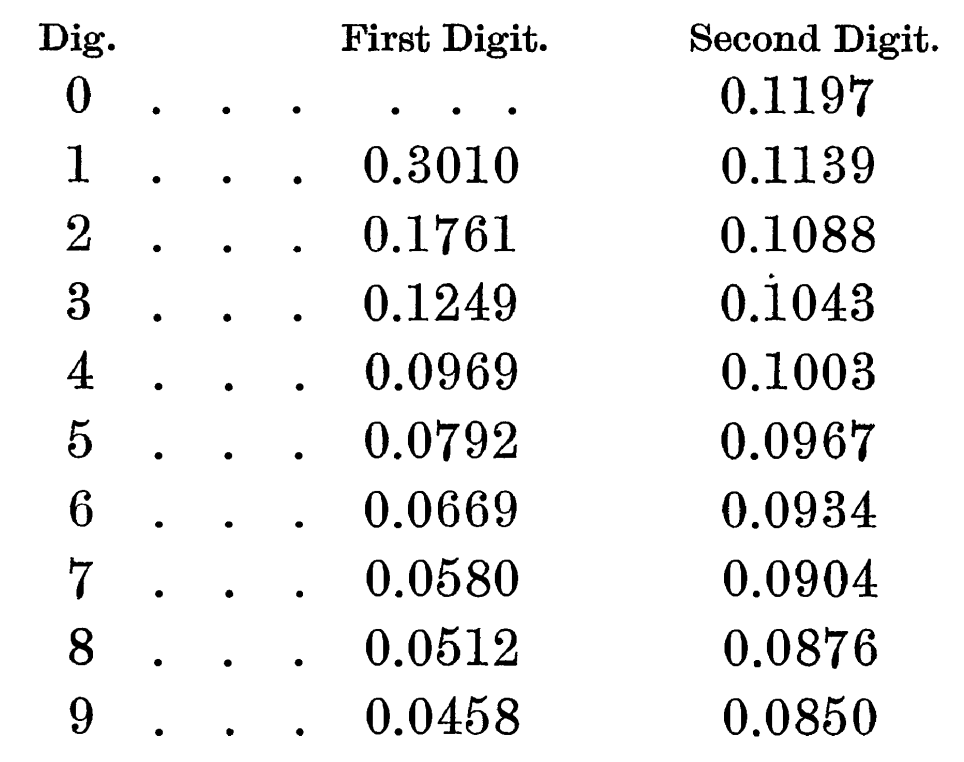
\includegraphics[scale=0.3]{newcomb1881.png}\footnote{\tiny{Newcomb (1881,40) - Note on the Frequency of Use of the Different Digits in Natural Numbers}}
  \end{center}
  \end{itemize}
\end{frame}

\begin{frame}{Ex. 3: \href{https://en.wikipedia.org/wiki/Benford\%27s_law}{Lei de Newcomb-Benford}}
  \begin{center}
  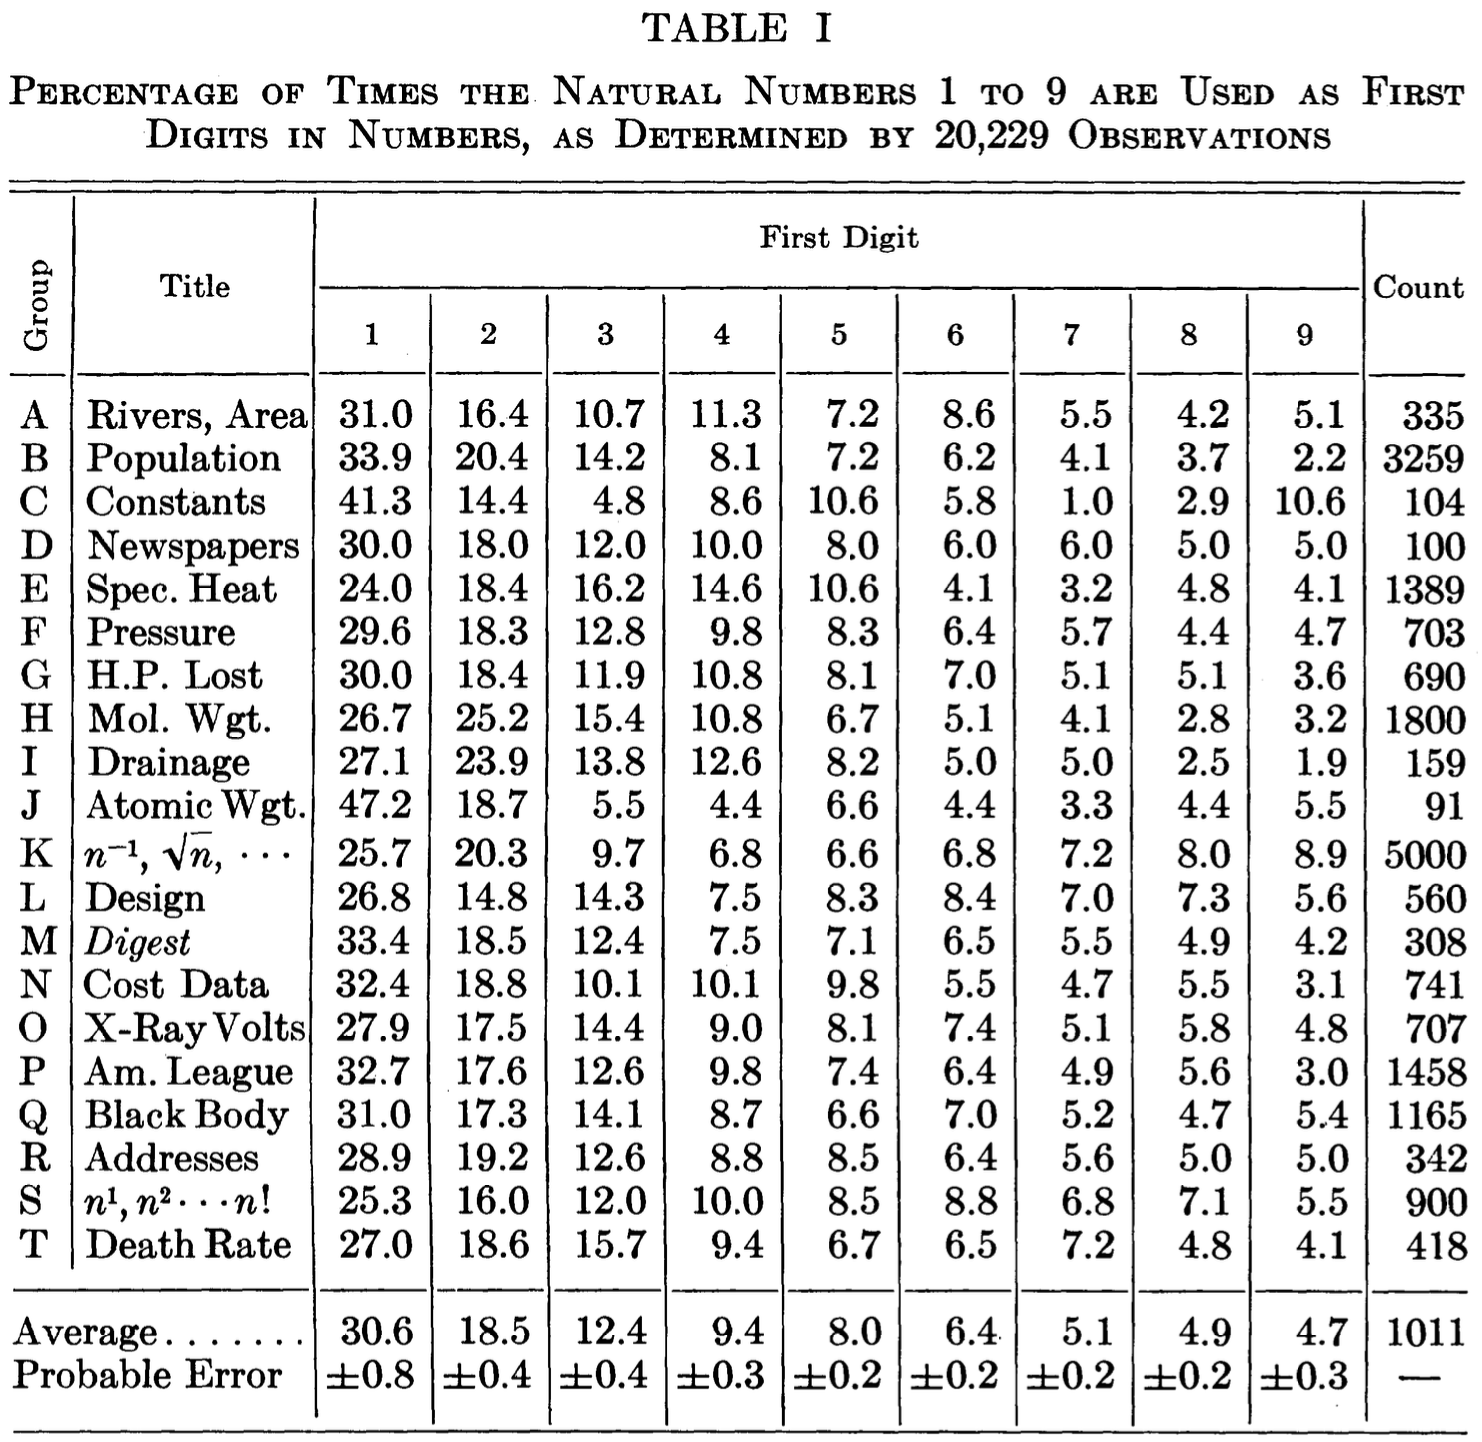
\includegraphics[scale=0.28]{benford1938.png}\footnote{\tiny{\href{https://en.wikipedia.org/wiki/Frank_Benford}{Frank Benford} (1938,553) - The Law of Anomalous Numbers}}
  \end{center}
\end{frame}

\begin{frame}{Ex. 3: \href{https://en.wikipedia.org/wiki/Benford\%27s_law}{Lei de Newcomb-Benford}}
  \begin{itemize}
    \item Frequência do dígito $a$ na 1$^a$ posição
  \end{itemize}
  \[F_a = \log_{10} \left( \frac{a+1}{a} \right)\]
  \[a=1,2,\ldots,9\]
\end{frame}


\begin{frame}[fragile]{Ex. 3: \href{https://en.wikipedia.org/wiki/Benford\%27s_law}{Lei de Newcomb-Benford}}
\fontsize{8pt}{8pt}\selectfont
\begin{knitrout}
\definecolor{shadecolor}{rgb}{0.969, 0.969, 0.969}\color{fgcolor}\begin{kframe}
\begin{alltt}
\hldef{Fa} \hlkwb{<-} \hlkwa{function}\hldef{(}\hlkwc{a}\hldef{)\{}\hlkwd{log}\hldef{((a}\hlopt{+}\hlnum{1}\hldef{)}\hlopt{/}\hldef{a,} \hlkwc{base} \hldef{=} \hlnum{10}\hldef{)\}}
\hlkwd{plot}\hldef{(}\hlkwd{Fa}\hldef{(}\hlnum{1}\hlopt{:}\hlnum{9}\hldef{))}
\end{alltt}
\end{kframe}

{\centering 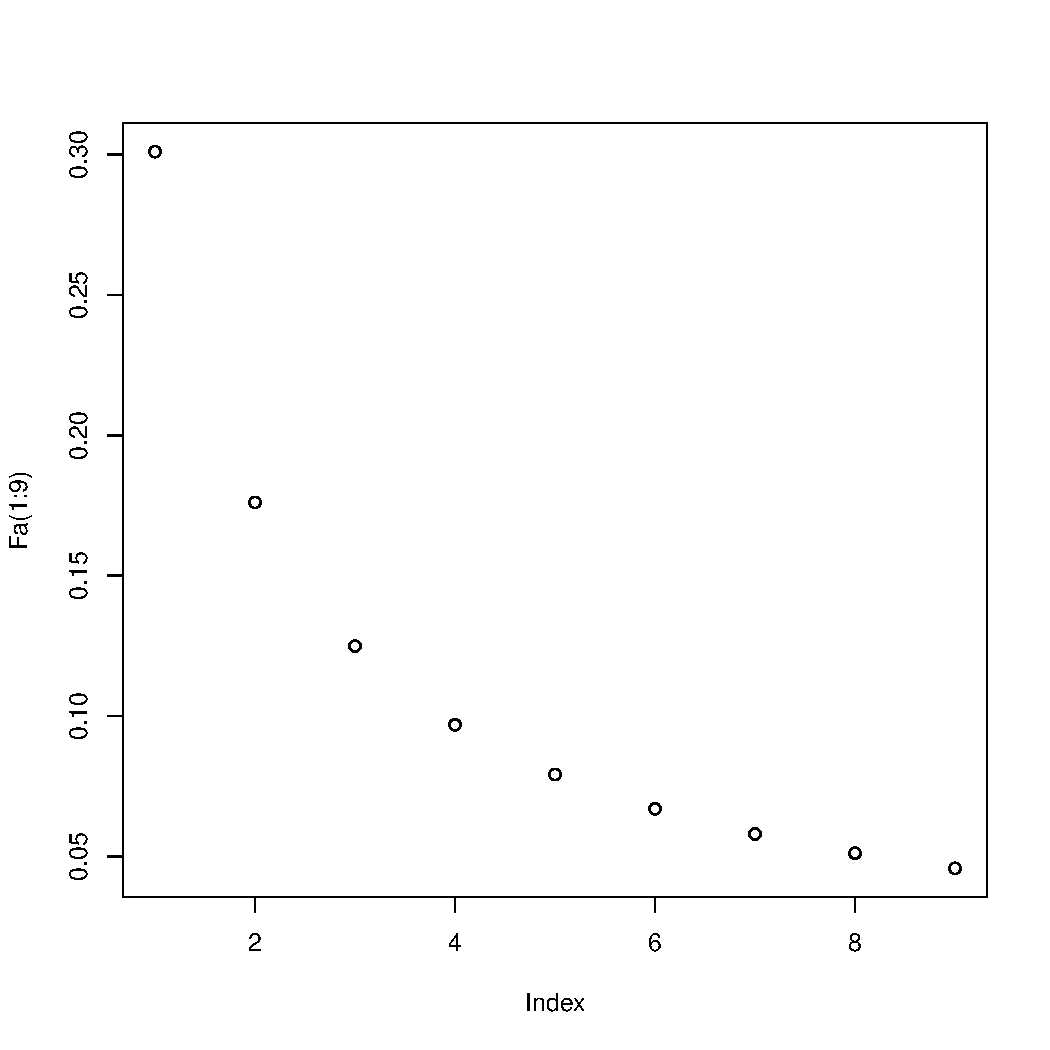
\includegraphics[width=.6\linewidth]{figure/Fa-1} 

}


\end{knitrout}
\end{frame}

\begin{frame}[fragile]{Ex. 3: \href{https://en.wikipedia.org/wiki/Benford\%27s_law}{Lei de Newcomb-Benford}}
 \begin{itemize}
    \item Frequência do dígito $b$ na 2$^a$ posição seguindo um dígito $a$ na 1$^a$ posição
  \end{itemize}
  \[F_{ab} = \frac{\log_{10} \left( \frac{ab+1}{ab} \right)}{\log_{10} \left( \frac{a+1}{a} \right)} \]
  \[ab = \{1,2,\ldots,9\} \times \{0,1,\ldots,9\}\]
\fontsize{8pt}{8pt}\selectfont
\begin{knitrout}
\definecolor{shadecolor}{rgb}{0.969, 0.969, 0.969}\color{fgcolor}\begin{kframe}
\begin{alltt}
\hldef{Fab} \hlkwb{<-} \hlkwa{function}\hldef{(}\hlkwc{a}\hldef{,}\hlkwc{b}\hldef{)\{}
  \hldef{ab} \hlkwb{<-} \hlkwd{as.numeric}\hldef{(}\hlkwd{paste0}\hldef{(a,b))}
  \hldef{fab} \hlkwb{<-} \hlkwd{log}\hldef{((ab}\hlopt{+}\hlnum{1}\hldef{)}\hlopt{/}\hldef{ab,} \hlkwc{base} \hldef{=} \hlnum{10}\hldef{)}\hlopt{/}\hlkwd{Fa}\hldef{(a)}
  \hlkwd{return}\hldef{(}\hlkwd{list}\hldef{(}\hlkwc{ab}\hldef{=ab,} \hlkwc{Fab}\hldef{=fab))}
\hldef{\}}
\hlkwd{Fab}\hldef{(}\hlnum{5}\hldef{,}\hlnum{0}\hldef{)}
\end{alltt}
\begin{verbatim}
## $ab
## [1] 50
## 
## $Fab
## [1] 0.1086137
\end{verbatim}
\end{kframe}
\end{knitrout}
\end{frame}

\begin{frame}[fragile]{Ex. 3: \href{https://en.wikipedia.org/wiki/Benford\%27s_law}{Lei de Newcomb-Benford}}
\fontsize{7pt}{7pt}\selectfont
\begin{knitrout}
\definecolor{shadecolor}{rgb}{0.969, 0.969, 0.969}\color{fgcolor}\begin{kframe}
\begin{alltt}
\hldef{grade} \hlkwb{<-} \hlkwd{expand.grid}\hldef{(}\hlnum{1}\hlopt{:}\hlnum{9}\hldef{,}\hlnum{0}\hlopt{:}\hlnum{9}\hldef{)}
\hldef{grade} \hlkwb{<-} \hlkwd{sort}\hldef{(}\hlkwd{as.numeric}\hldef{(}\hlkwd{paste0}\hldef{(grade[,}\hlnum{1}\hldef{],grade[,}\hlnum{2}\hldef{])))}
\hldef{prob} \hlkwb{<-} \hlkwd{data.frame}\hldef{(}\hlkwc{grade}\hldef{=grade,} \hlkwc{Fab}\hldef{=}\hlnum{NA}\hldef{)}
\hldef{k} \hlkwb{<-} \hlnum{0}
\hlkwa{for}\hldef{(i} \hlkwa{in} \hlnum{1}\hlopt{:}\hlnum{9}\hldef{)\{}
  \hlkwa{for}\hldef{(j} \hlkwa{in} \hlnum{0}\hlopt{:}\hlnum{9}\hldef{)\{}
    \hldef{k} \hlkwb{<-} \hldef{k}\hlopt{+}\hlnum{1}
    \hldef{prob[k,}\hlnum{2}\hldef{]} \hlkwb{<-} \hlkwd{Fab}\hldef{(i,j)}\hlopt{$}\hldef{Fab}
  \hldef{\}}
\hldef{\}}
\hlkwd{plot}\hldef{(prob[,}\hlnum{1}\hldef{], prob[,}\hlnum{2}\hldef{],} \hlkwc{xlab} \hldef{=} \hlsng{''}\hldef{,} \hlkwc{ylab}\hldef{=}\hlsng{''}\hldef{)}
\end{alltt}
\end{kframe}

{\centering 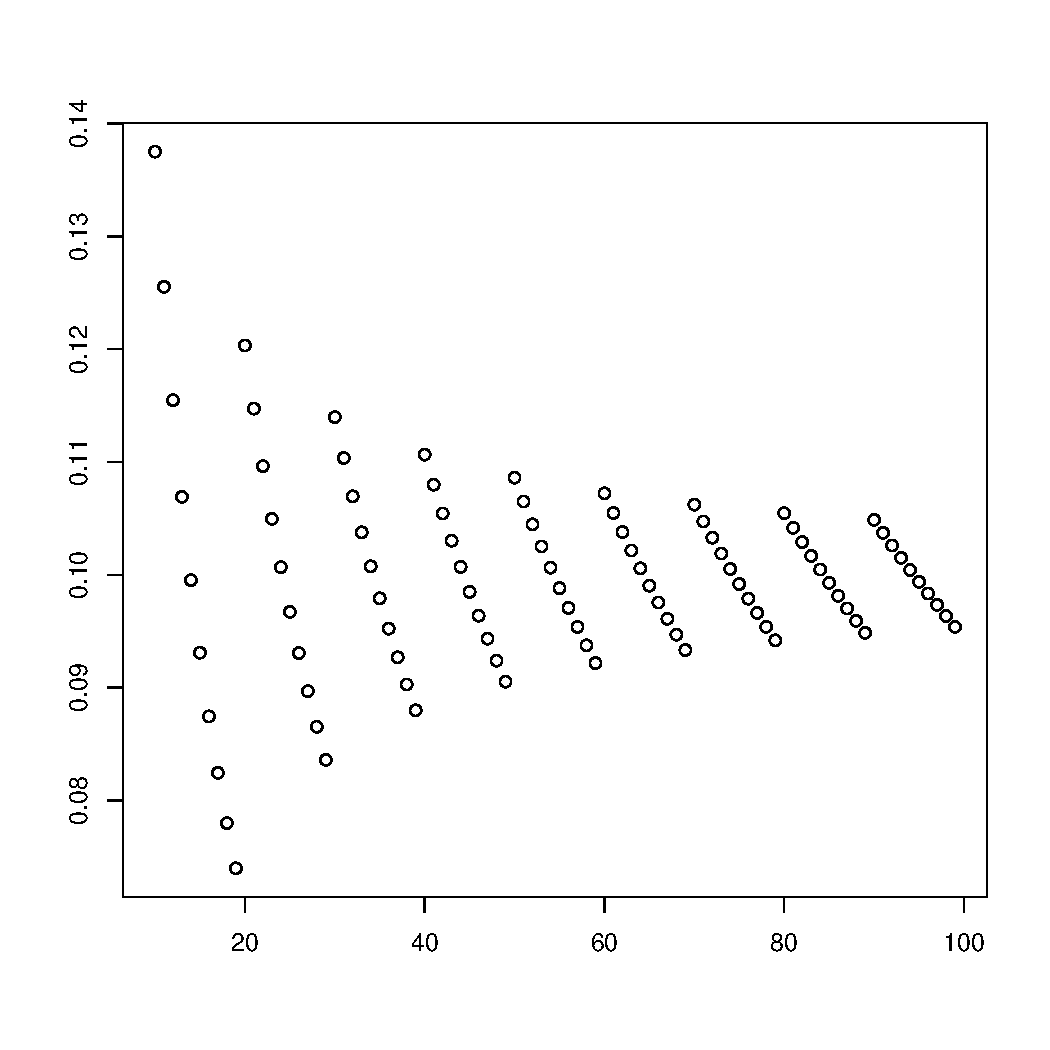
\includegraphics[width=.5\linewidth]{figure/Fab_plot-1} 

}


\end{knitrout}
\end{frame}

\begin{frame}[fragile]{Ex. 3: \href{https://en.wikipedia.org/wiki/Benford\%27s_law}{Lei de Newcomb-Benford}}
\fontsize{7pt}{7pt}\selectfont
\begin{knitrout}
\definecolor{shadecolor}{rgb}{0.969, 0.969, 0.969}\color{fgcolor}\begin{kframe}
\begin{alltt}
\hlkwd{library}\hldef{(benford.analysis)}
\hlkwd{data}\hldef{(corporate.payment)}
\hldef{bfd} \hlkwb{<-} \hlkwd{benford}\hldef{(corporate.payment}\hlopt{$}\hldef{Amount)}
\hlkwd{plot}\hldef{(bfd)}
\end{alltt}
\end{kframe}

{\centering 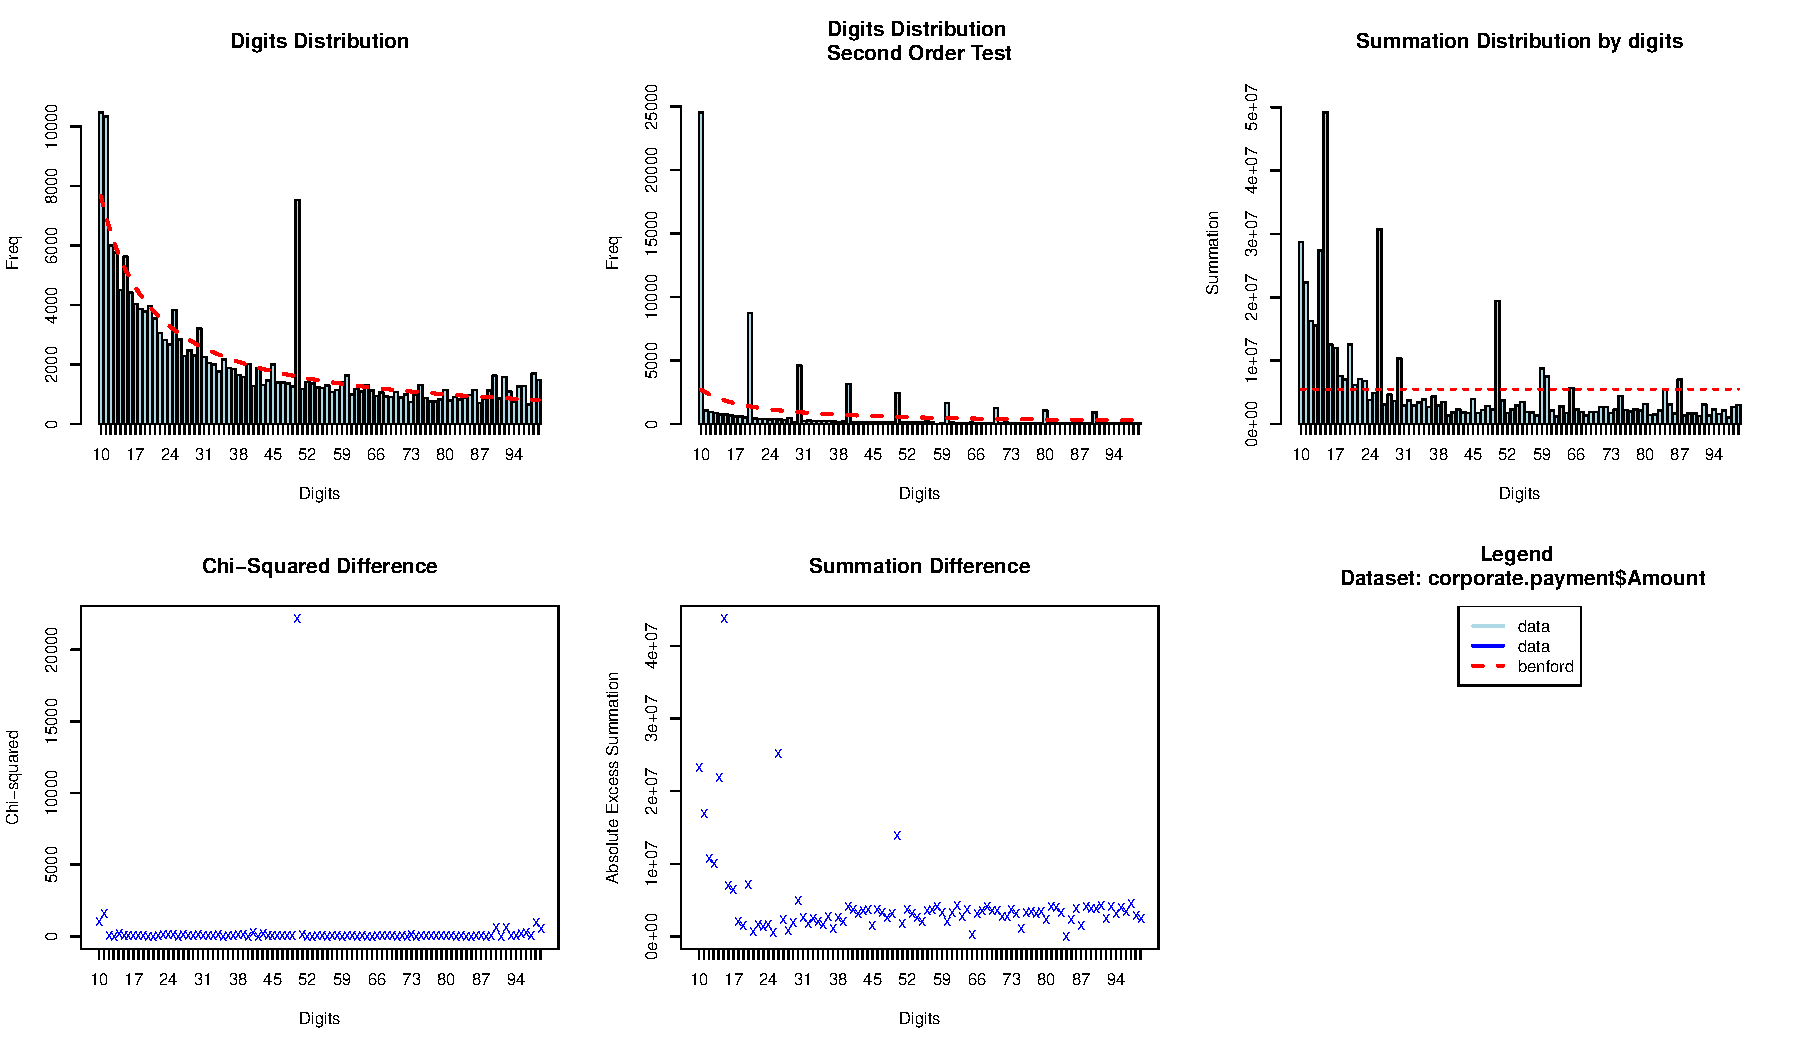
\includegraphics[width=.8\linewidth]{figure/lib_benford-1} 

}


\end{knitrout}
\end{frame}


\begin{frame}[fragile]{Ex. 4: \href{https://cran.r-project.org/web/packages/voice/index.html}{\texttt{voice}}}
  \begin{itemize}
    \item \href{https://github.com/filipezabala/voice/}{\texttt{voice}}: ferramentas para análise de voz, reconhecimento de falantes e inferência de humor
  \end{itemize}
  \pause
\fontsize{7pt}{7pt}\selectfont
\begin{knitrout}
\definecolor{shadecolor}{rgb}{0.969, 0.969, 0.969}\color{fgcolor}\begin{kframe}
\begin{alltt}
\hlkwd{library}\hldef{(voice)}
\hldef{path2wav} \hlkwb{<-} \hlkwd{list.files}\hldef{(}\hlkwd{system.file}\hldef{(}\hlsng{'extdata'}\hldef{,} \hlkwc{package} \hldef{=} \hlsng{'wrassp'}\hldef{),}
                       \hlkwc{pattern} \hldef{=} \hlkwd{glob2rx}\hldef{(}\hlsng{'*.wav'}\hldef{),} \hlkwc{full.names} \hldef{=} \hlnum{TRUE}\hldef{)}
\hldef{E} \hlkwb{<-} \hldef{dplyr}\hlopt{::}\hlkwd{tibble}\hldef{(}\hlkwc{subject_id} \hldef{=} \hlkwd{c}\hldef{(}\hlnum{1}\hldef{,}\hlnum{1}\hldef{,}\hlnum{1}\hldef{,}\hlnum{2}\hldef{,}\hlnum{2}\hldef{,}\hlnum{2}\hldef{,}\hlnum{3}\hldef{,}\hlnum{3}\hldef{,}\hlnum{3}\hldef{),} \hlkwc{wav_path} \hldef{= path2wav)}

\hlcom{# resume o áudio por sujeito}
\hldef{voice}\hlopt{::}\hlkwd{tag}\hldef{(E,} \hlkwc{groupBy} \hldef{=} \hlsng{'subject_id'}\hldef{)}
\end{alltt}
\begin{verbatim}
## # A tibble: 3 x 7
##   subject_id f0_tag_mean f0_tag_sd f0_tag_vc f0_tag_median f0_tag_iqr f0_tag_mad
##        <dbl>       <dbl>     <dbl>     <dbl>         <dbl>      <dbl>      <dbl>
## 1          1        85.1      15.3     0.180          78.3       26.8      11.9 
## 2          2        84.6      14.9     0.176          76.4       28.3       7.97
## 3          3        81.0      14.6     0.180          75.6       21.6       8.68
\end{verbatim}
\end{kframe}
\end{knitrout}
\end{frame}


\begin{frame}{Ex. 5: Tempo de operação de ATMs}
	\begin{center}
    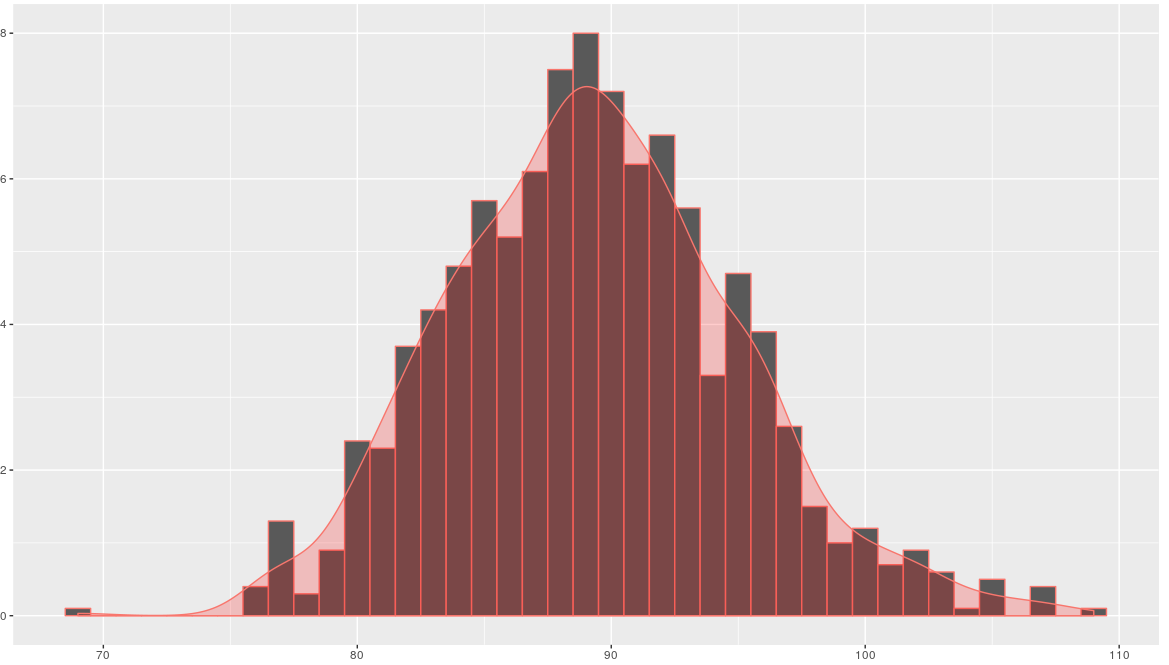
\includegraphics[scale=0.25]{horasOp.png}
  \end{center}
\end{frame}


\section{Publicidade de dados PÚBLICOS}
\begin{frame}{\secname}
  \begin{itemize}
    \item \href{http://www.planalto.gov.br/ccivil_03/_ato2011-2014/2011/lei/l12527.htm}{Brasil (2011) Lei 12.527 de 18/11/2011}
    \item \href{http://www.planalto.gov.br/ccivil_03/_ato2011-2014/2012/Decreto/D7724.htm}{Brasil(2012) Brasil. Decreto 7.724 de 16/05/2012}
	\end{itemize}
	\begin{center}
  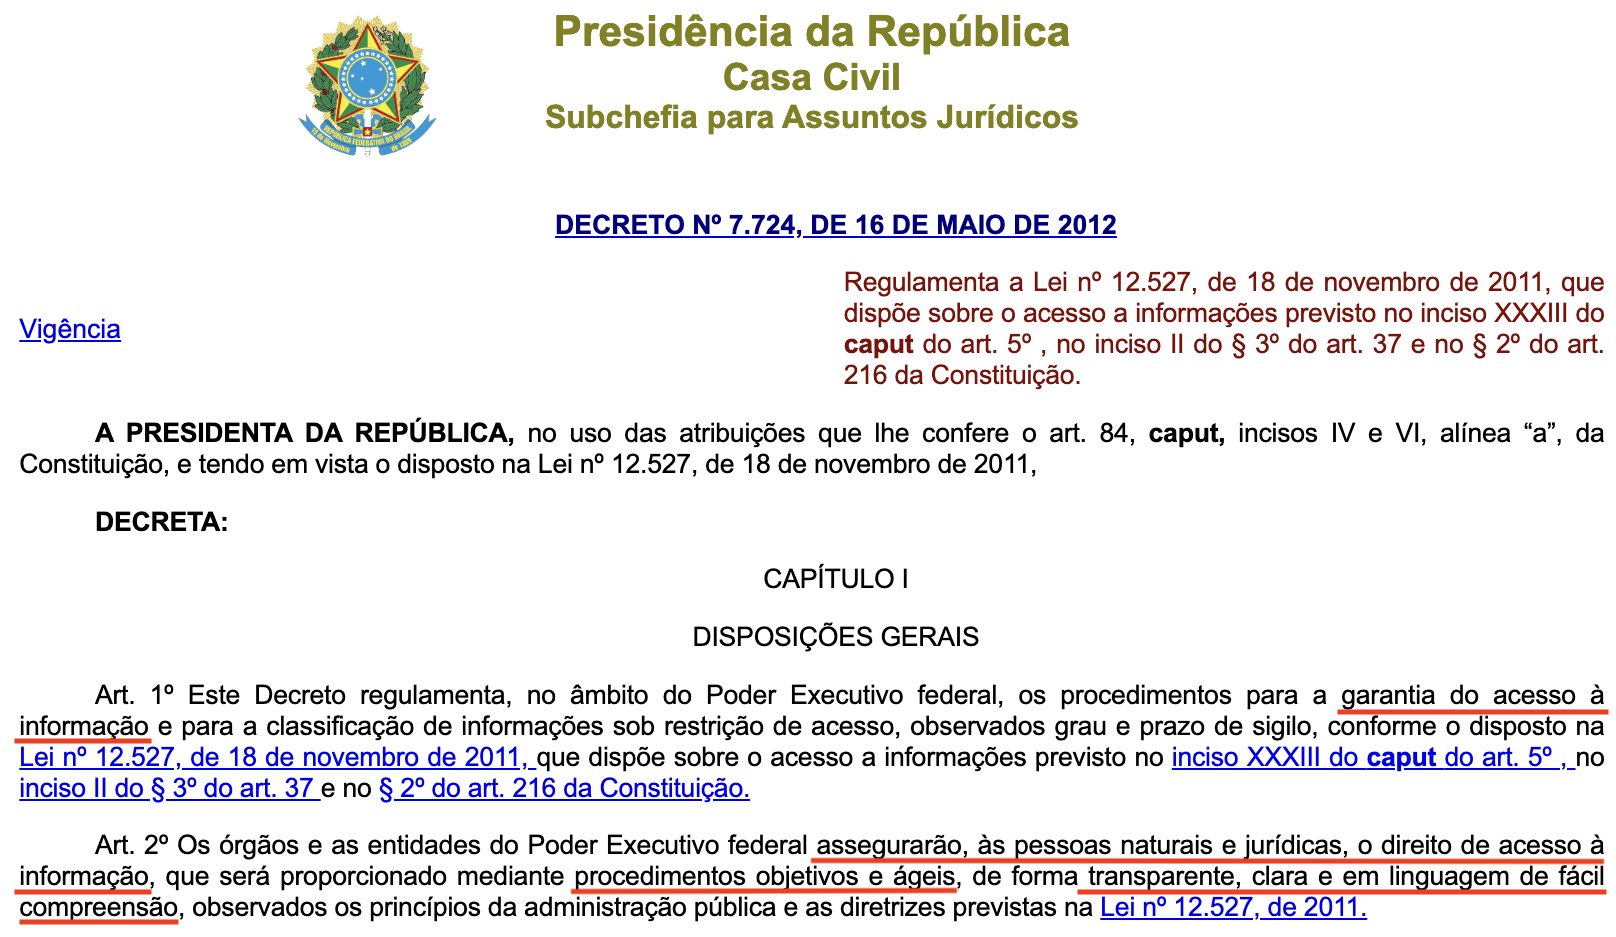
\includegraphics[scale=0.3]{lai12.png}
  \end{center}
\end{frame}

\begin{frame}{\secname}
\blfootnote{\tiny{\href{https://www.artificiallawyer.com/2019/06/04/france-bans-judge-analytics-5-years-in-prison-for-rule-breakers/}{Artificial Lawyer (2019-06-04) - France Bans Judge Analytics, 5 Years In Prison For Rule Breakers}}}
\begin{figure}
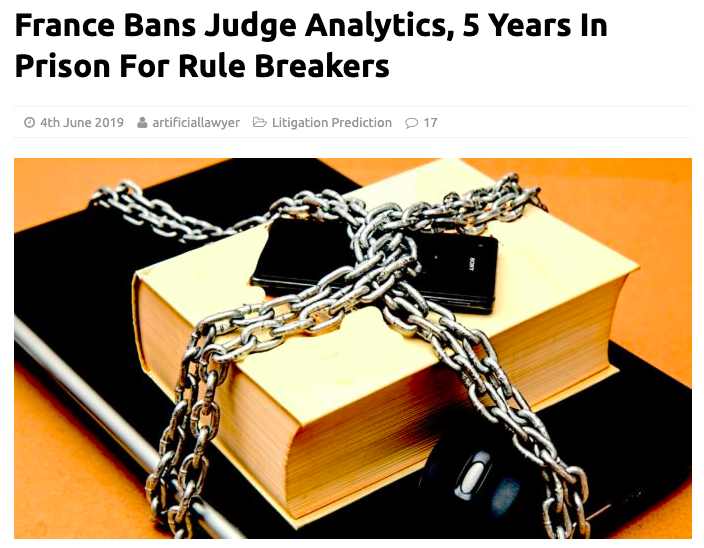
\includegraphics[scale=0.35]{franca}
\end{figure}
\end{frame}

\section{Privacidade de dados PESSOAIS}
\begin{frame}{\secname}
  \begin{itemize}
    \item \href{http://www.dbis.informatik.hu-berlin.de/fileadmin/lectures/SS2011/VL_Privacy/Differential_Privacy.pdf}{Dwork (2006) - Differential Privacy}
    \pause
    \item \href{https://books.google.com.br/books/about/Weapons_of_Math_Destruction.html?id=CxD-DAAAQBAJ&redir_esc=y}{O'Neil (2016) - Weapons of Math Destruction}
	\end{itemize}
	\begin{center}
  
\includegraphics[scale=0.3]{weapons.jpg}
  \end{center}
\end{frame}

% \section{Privacidade de dados PESSOAIS}
\begin{frame}{\secname}
  \begin{itemize}
    \item \href{https://www.planalto.gov.br/ccivil_03/_ato2015-2018/2018/lei/l13709.htm}{Lei 13.709, de 14 de agosto de 2018}
	\end{itemize}
\bigskip
	\begin{center}
  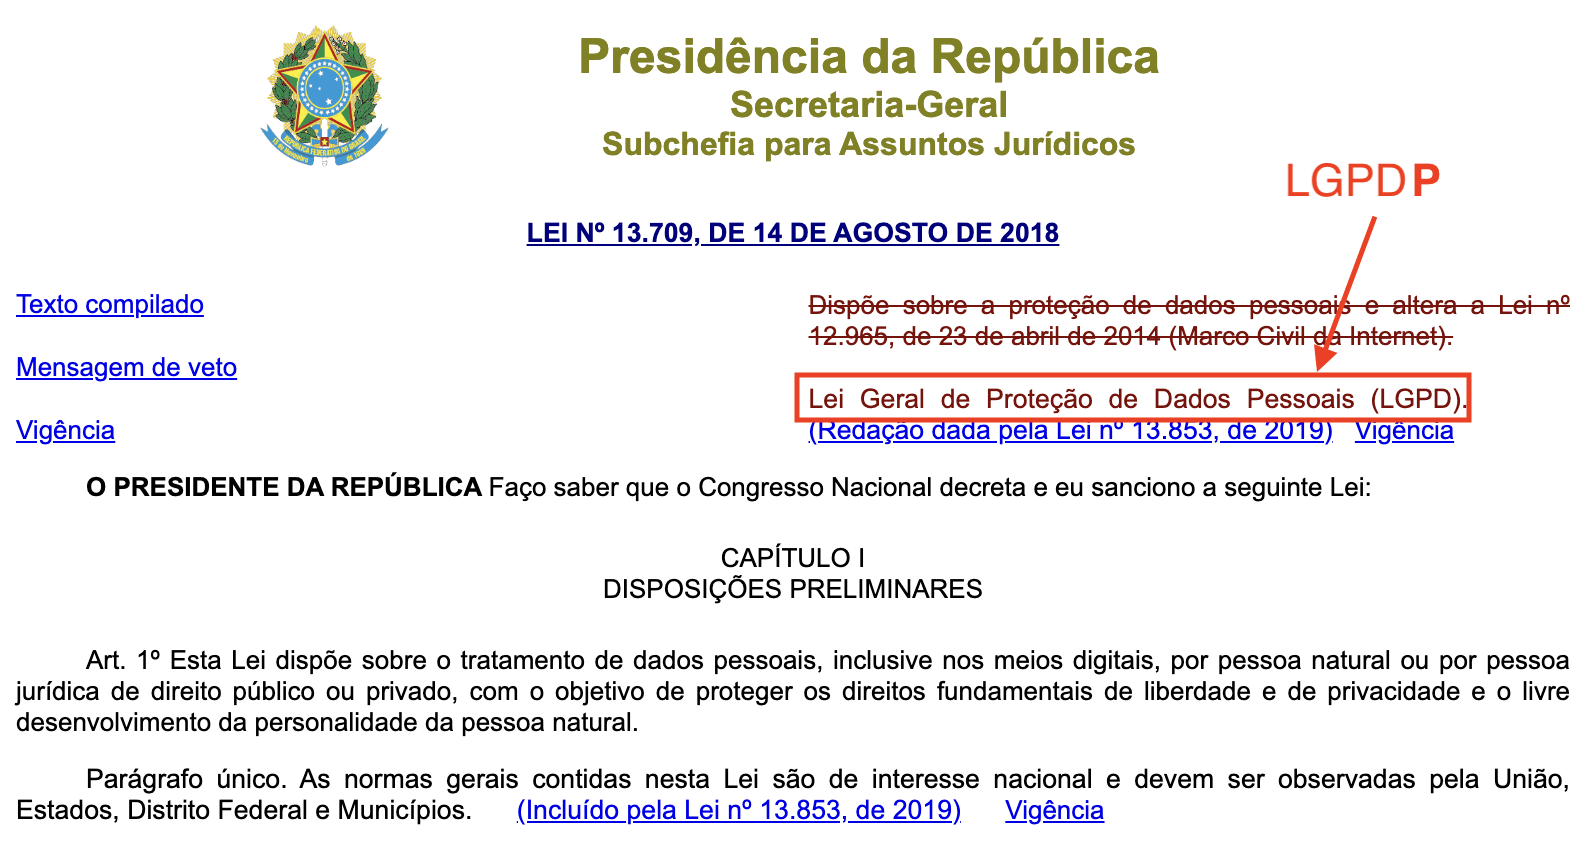
\includegraphics[scale=0.3]{lgpdp.png}
  \end{center}
\end{frame}

\section{Para saber mais}
\begin{frame}{\secname}
\fontsize{9pt}{9pt}\selectfont
  \begin{enumerate}
  \itemsep.5em
  	\item \href{https://www.jstor.org/stable/2369148}{Newcomb (1881) - Note on the Frequency of Use of the Different Digits in Natural Numbers}
  	\item \href{http://www.brunodefinetti.it/Opere/funzioneCaratteristica.pdf}{De Finetti (1930) - Funzione Caratteristica di un Fenomeno Aleatorio}
  	\item \href{https://isidore.co/misc/Physics\%20papers\%20and\%20books/Zotero/storage/ZEBWDL73/Benford\%20-\%201938\%20-\%20The\%20Law\%20of\%20Anomalous\%20Numbers.pdf}{Benford (1938) - The Law of Anomalous Numbers}
  	\item \href{https://archive.org/details/mathematicsimagi00kasnrich}{Kasner and Newman(1940) - Mathematics and the
Imagination}
  	\item \href{https://doi.org/10.1017/CBO9780511569647}{Aitchison \& Dunsmore (1975) - Statistical Prediction Analysis}
  	\item \href{https://www.sciencedirect.com/science/article/abs/pii/B9780124381506500182}{Box (1979) - Robustness in the Strategy of Scientific Model Building}
    \item \href{https://link.springer.com/book/10.1007/978-1-4612-3894-2}{Ghosh (1988) - Statistical Information and Likelihood - A collection of critical essays by Dr. D. Basu}
    \item \href{https://doi.org/10.1201/9780203742310}{Seymour Geisser (1993) - Predictive Inference - An Introduction}
    \item \href{https://projecteuclid.org/euclid.ss/1009213726}{Breiman (2001) - Statistical Modeling: The Two Cultures}
    \item \href{https://doi.org/10.11606/D.45.2009.tde-01032021-140004}{Zabala (2009) - Desempate Técnico}
	\end{enumerate}
\end{frame}


% \section{Para saber mais}
\begin{frame}{\secname}
\fontsize{9pt}{9pt}\selectfont
  \begin{enumerate}
  \setcounter{enumi}{10}
  \itemsep.5em
  	\item \href{https://web.williams.edu/Mathematics/sjmiller/public_html/cmu/21-499/handouts/benford/Fewster_SimpleExplanationBenfordLaw.pdf}{Fewster (2009) - A Simple Explanation of Benford’s Law}
  	\item \href{https://ww2.esmarn.tjrn.jus.br/revistas/index.php/revista_direito_e_liberdade/article/view/732}{Zabala \& Silveira (2014) - Jurimetria: Estatística Aplicada ao Direito}
  	\item \href{https://doi.org/10.1017/9781139236003}{Clarke \& Clarke (2018) - Predictive Statistics - Analysis and Inference Beyond Models}
    \item \href{https://otexts.com/fpp2/}{Hyndman \& Athanasopoulos (2018) - Forecasting: Principles and Practice}
    \item \href{https://arxiv.org/abs/2001.00476}{Zabala \& Silveira (2019) - Decades of Jurimetrics}  
  	\item \href{http://www.rizbicki.ufscar.br/ame/}{Izbicki \& Santos (2020) - Aprendizado de Máquina: uma abordagem estatística}
    \item \href{https://www.youtube.com/@filipezabala}{Zabala (2020) - Vídeos: Ciência de dados em software livre}
  	\item \href{https://github.com/filipezabala/cddesl}{Zabala (2020) - Código: Ciência de dados em software livre}
  	\item \href{https://doi.org/10.1016/j.physa.2020.125626}{Azevedo et al (2021) - A Benford’s Law based methodology for fraud detection in social welfare programs - Bolsa Familia analysis}
  	\item \href{https://CRAN.R-project.org/package=voice}{Zabala (2023). voice: Tools for Voice Analysis, Speaker Recognition and Mood Inference}
	\end{enumerate}
\end{frame}

\end{document}
